%\documentclass[paper]{geophysics}
\documentclass[manuscript,revised]{geophysics}


% An example of defining macros
\newcommand{\rs}[1]{\mathstrut\mbox{\scriptsize\rm #1}}
\newcommand{\rr}[1]{\mbox{\rm #1}}

\newcommand{\psm}{\textit{PSM} }
\newcommand{\twod}{two-dimensional }
\newcommand{\thrd}{three-dimensional }

\usepackage{lineno}

% printing options
%\usepackage{pgfpages}
%\pgfpagesuselayout{4 on 1}[letterpaper,border shrink=5mm]


\begin{document}

\title{tmp title: MUSC source}

\renewcommand{\thefootnote}{\fnsymbol{footnote}} 

\ms{GEO-Example} % manuscript number

\address{
\footnotemark[1]LUNAM-IFSTTAR, \\
\footnotemark[2]OSUNA \\
\footnotemark[1]LPGN, \\}
\author{Damien Pageot\footnotemark[1]\footnotemark[2], Donatienne Leparoux\footnotemark[1], Mathieu Le Feuvre\footnotemark[1], Olivier Durand\footnotemark[1] and Yann Capdeville\footnotemark[3]}

\footer{Example}
\lefthead{Dellinger \& Fomel}
\righthead{\emph{Geophysics} example}

\maketitle

\begin{abstract}
\end{abstract}

\modulolinenumbers[5]
\linenumbers

% ## INTRODUCTION
\section{Introduction}

% #### Nature and scope of the problem
%\noindent Since decades, geophysicists develop numerical inversion and imaging methods for seismic measurements (receiver function analysis  \citep{Ammon_1991_IRE}, ray-based methods \citep{Jones_PRM_2013}, finite-frequency tomography \citep{Montelli_FFT_2004}, inversion-based methods \citep{Virieux_FWI_2009}) to determine the structures and the physical properties of the Earth at several scales as subsurface (civil engineering), crustal, regional or global. These methods, like Full Waveform Inversion (FWI), are still in development and are mostly validated using synthetic data which are generally computed using the same wave propagation modeling engine used in the inverse problem process. In other terms, the synthetic data are computed with some assumptions (for example acoustic approximation or \twod) which are the same in the inverse problem. Although, this \textit{inverse crime} \citep{Wirgin_TIC_2004} is particularly useful to validate an algorithm in its early development stage, it does not allow to assess the efficiency of the method for real seismic data. Moreover, because no one known precisely the Earth interior, it is difficult to evaluate the capacity of a method to recover physical parameters and structures from real seismic data which can lead sometimes to geological interpretation of numerical artifacts \citep{Morozov_ARF_2004}. Thus, it is necessary to add a step for which imaging methods will be tested for experimental seismic measurements obtained under controlled conditions.

\noindent Since the early developments of seismic imaging methods in the middle of 20th century, approaches and algorithms innovations are still proposed in current research projects. The improvements deal with both the qualitative imaging techniques like migration (e.g. \citet{Berkhout_MSS_2012,Guofeng_GPU_2013}), novel applications of quantitative imaging methods such as the first arrival tomography (e.g. \citet{Bohm_CWS_2015}), or even more recent approaches like the Full Waveform Inversion (e.g. \citet{Perez_AWI_2014}, see \citet{Virieux_FWI_2009} for a revue of this last decade). The refinements are proposed for different scales like near surface applications for civil engineering topics or more deeper investigation for example for oil prospection or crustal imaging at regional or global scales. They are mostly validated by using synthetic data, for example with well known shared benchmark (like the Marmousi case). However, the synthetic data are generally computed using the same wave propagation modeling engine used in the inverse problem process. In other terms, the synthetic data are computed with some assumptions which are the same in the inverse problem, for example the approximation of acoustic propagation, a 2D space medium, or a 2D line source. This approach, called \textit{inverse crime} \citep{Wirgin_TIC_2004} is particularly useful for validating an algorithm in its early development stage but does not take into account the artefacts that can be due to the assumptions of the direct problem. Some authors tackle this issue by providing 3D data which are inverted with a 2D approach or other restrictive assumptions (e.g ). But also in this case, the approach does not allow to assess the efficiency of the method for real seismic data. Moreover, because no one knows precisely the Earth interior, it is difficult to evaluate the capacity of a method to recover physical parameters and structures from real seismic data which can lead sometimes to geological misinterpretation due to numerical artifacts \citep{Morozov_ARF_2004}. Thus, it is necessary to add a step for which imaging methods will be tested for experimental seismic measurements obtained under controlled conditions.

\noindent The best way to satisfy this need is to use Physical Small Scale Modeling Methods (noted \psm subsequently). \psm were used since several years to study the propagation of waves in various media with several stage of complexity, from acoustic wave propagation in homogeneous media to elastic wave propagation in \thrd heterogeneous anisotropic media \citep{Rieber_EWP_1936,Howes_SMS_1953,Hilterman_TDM_1970,French_MRP_1974,Bishop_LVM_1985,Pratt_FWI_1999,Favretto_NMT_2013,Sarkar_TPM_2003,Isaac_SMS_1999}, and allow to generate experimental seismic data under well-controlled conditions. In this way, recent studies have been conducted to simulate multi-sources and multi-receivers through piezo-electric transducers \citep{Wong_SPM_2009}. An alternative approach consists in using the laser interferometry as the receiver system, as done in the MUSC Laboratory \citep{Bretaudeau_SSA_2008b,Bretaudeau_SSM_2011,Bretaudeau_FWI_2013}, \textit{Mesure Ultrasonore Sans Contact} in French, is one of them. This technology, by avoiding the contact of the receivers on the model, allows to by-pass the coupling issue of transducers that is difficult to model. In this way,the MUSC laboratory is designed to simulate (1) wide-angle on-shore acquisitions modeling both body waves and surface waves, (2) automatic multisource-multireceiver measurements with a high-productivity, (3) high-precision source-receiver positioning and (4) high-precision recording of absolute surface displacement without coupling effects. 

% #### State the objectives
\noindent Our objective here is to increase the potential of the MUSC system as a reliable tool for generating experimental data which will be distributed in the scientific community. 
\noindent Thus, we present two studies of experimental data in order to : 1) quantitatively refine the comparison between numerical and experimental data by taking into account the 3D/2D geometrical spreading effects through an alternative way and 2) identify the reproducibility of the source impact and, consequently, data repeatability. These approaches will complete the knowledge of the system and facilitate the achievement of massive multi-source and multi-receiver data simulating subsurface seismic experimental campaigns. Moreover, they provide quantitative informations about the data quality for geophysicists who need to use them measurement based on reduced scale model. 

% #### Describe the method of investigation
\noindent In order to achieve these objectives, we used a seismic wave modeling code based on the Spectral Element Method \citep{Komatitsch_SEM_1998,Komatitsch_ISM_1999,Komatitsch_SEM_2005,Festa_PML_2005} that allow to provide numerical signals as reference data for comparison. The Spectral Element Method (SEM) has several advantages compared to finite differences and finite elements, such as: (1) a weak formulation which can naturally take into account the free surface, (2) an explicit scheme in time domain facilitating parallelization and reducing the computational cost, (3) a spatial discretization (mesh) convenient for the representation of complex environments and (4) high precision results and low numerical dispersion.

% #### Describe the principal results of the investigation

\noindent The numerical characteristics of the code used are described in a first part below. Afterwards, the specificities of the MUSC system are explained, followed by the presentation of the models used. Finally The two coupled studies on experimental data are detailed, in the respective aims (1) of refining the comparison between numerical and experimental data by taking into account the geometrical spreading effects between \twod and \thrd data through an alternative way, and (2) of identifying the reproducibility of the source impact to validate the data reproducibility.


% ## METHODS
\section{Methods}

% #### Spectral Element Method
\subsection{Numerical modeling: Spectral Element Method}

%La méthode des différence-finies (DF ) est la méthode de résolution des EDP la plus rependue et développée en sciences de la Terre de par sa simplicité (relative), sa robustesse et son cout numérique faible (Virieux, 1986; Levander, 1988; Bohlen & Saenger, 2006). La méthode des DF permet la discrétisation du domaine sur une grille cartésienne et, généralement, avec un pas de grille régulier et approxime les valeurs des dérivées partielles par un développement de Taylor à un ordre dépendant de la précision souhaitée de la solution. Cependant, la méthode des DF, malgré sa popularité, souffre de quelques inconvénients pouvant s'avérer handicapant dans certaines configurations. Tout d'abord, le maillage sous forme de grille cartésienne pose un problème dans des configurations où une représentation réaliste de la topographie serait nécessaire, amenant alors à sur-échantillonner le milieu avec un pas de grille plus petit afin de pouvoir reproduire correctement la topographie. Une autre difficulté est liée à l’ordre du développement de Taylor entraînant une extension du schéma numérique, en nombre de nœuds de grille, au fur et à mesure qu'il augmente (Levander, 1988). La méthode particulière mixed-grid pour la modélisation en domaine fréquentiel (Jo et al., 1996; Hustedt et al., 2004) sera présentée dans la section suivante.

%La méthode des éléments finis (EF) se propose de résoudre les systèmes d’EDP en se basant sur une forme variationnelle du problème à résoudre. Le domaine est généralement discrétisé, en 2D, par des éléments triangulaires pour lesquels chaque nœud est associé à une fonction de base polynomiale choisie de manière à obtenir la matrice inversible la plus creuse possible. Les EF permettent aussi bien des maillages réguliers qu'irréguliers les rendant ainsi tout à fait adaptés à la discrétisation de milieu présentant des interfaces complexes et de la topographie. Les EF peuvent être divisés en deux sous catégories : les EF continus, pour lesquels les échanges d’informations entre les cellules se font par les nœuds qui sont communs entre cellules voisines, et les EF discontinus, pour lesquels les nœuds sont propres à chaque cellules et où les échanges d’informations entre cellules voisines se font par des flux numériques aux interfaces. Le schéma des Galerkin discontinus (Cockburn, 2003), qui sera décrit par la suite, appartient à cette deuxième catégorie d’EF. 

%La méthode des éléments spectraux (ES ) (Faccioli et al., 1997; Komatisch et al., 1998; Capdeville et al., 2003) est une méthode de résolution des EDP répandue notamment dans le domaine de la tomographie globale et régionale grâce à ses caractéristiques permettant la mise en place d’un maillage grossier du milieu. Le méthode des ES est une variante des EF utilisant des ordres d’interpolation polynomiaux élevés amenant à un taux de convergence spectrale à mesure que l’ordre d’interpolation augmente. Cette approche permet d’obtenir une matrice de masse diagonale qui ne nécessitera par conséquent aucune inversion. Cependant, le maillage, qui est une clé du succès des ES, est également sa principale limitation. Composé de quadrangle en 2D et de parallélépipèdes en 3D, le maillage n’est pas aussi adaptés que les EF aux milieux présentant des topographies et interfaces complexes. Des développements récents basés sur les principes d’homogénéisation visent actuellement à s'affranchir de cette limite liée au maillage (Capdeville et al., 2010).


\noindent Various numerical methods exist to resolve the equation of motion in arbitrary elastic media. The most widely used for seismic applications is the Finite-Differences (FD) method \citep{Virieux_PSV_1986,Levander_PSV_1988,Robertsson_FDM_1994,Pratt_EWM_1990,Stekl_VEM_1998,Saenger_FDM_2004} which estimates each derivative on a regular Cartesian grid using a Taylor development \citep{Moczo_FDM_2004} of order \textit{n}. FD is simple to implement and robust but quickly shows some limitations. First the Cartesian grid is defined by the minimum propagated wavelength ($\lambda_{min}$) in the full medium which conducts to a very small spatial step in case of low velocities zones it is usually the case for subsurface issues. Moreover, \citet{Saenger_FDM_2000} show that 60 points by wavelength ($\lambda$) are needed to model propagation of Rayleigh wave in order $n=2$ where only 15 points by $\lambda$ are required to model propagation of body waves which increases drastically the numerical cost in case of near-surface modeling experiment. Second, the Cartesian grid does not provide a suitable tool to reproduce properly complex topography and interfaces. 

\noindent To overcome this limit, one can use the Finite-Elements Method (FEM) which is another popular method used for wave propagation modeling \citep{Lysmer_FEM_1972,Seron_FEM_1990,Hulbert_FEM_1990}. FEM is based on a variational formulation of the equation of motion and gives a continuous approximate solution in space using polynomial basis functions defined on each node of each cell of the mesh. The natural boundary conditions of FEM is the free surface and the triangular (in 2D) or tetraedric (in 3D) unstructured meshes are well adapted to complex media and topography. However, low polynomial basis are inadequate with fine spatial discretization and the required discretization to obtain precise and non-dispersive solution is numerically costly. 

\noindent Parallel, at the end of the 20th century, the Spectral Element Method (SEM), widely used in fluid dynamics \citep{Patera_SEM_1984,Korczak_SEM_1986,Karniadakis_FEM_1989}, has been adapted to seismic wave propagation \citep{Komatitsch_SEM_1998,Komatitsch_ISM_1999,Komatitsch_SEM_2005,Festa_PML_2005}. The SEM is a variant of FEM based upon a high-order piecewise polynomial approximation of the weak formulation of the wave equation which leads to a spectral convergence ratio as the interpolation order increases. 

\noindent In this method, the wave-field is represented in terms of high-degree Lagrange interpolants, and integrals are computed based upon Gauss-Lobatto-Legendre (gll) quadrature. This combination leading to a perfectly diagonal mass matrix leads in turn to a fully explicit time scheme which leads itself very well to numerical simulations on parallel computers.

\noindent SEM inherits the flexibility and the natural free surface condition of the FEM \citep{Tromp_SEM_2008}. The typical element size that is required to generate an accurate mesh is of the order of $\lambda$, $\lambda$ being the smallest wavelength of waves traveling in the model.  Models are meshed with quadrangles (2D) and hexaedras (3D) using the open-source software package GMSH \citep{Geuzaine_MSH_2009}. It is particularly well suited to handle complex geometries and interface matching conditions \citep{Cristini_SEM_2012}. In order to simulate infinite or semi-infinite domain, SEM can use Perfect Match Layers boundary conditions \citep{Berenger_PML_1994,Festa_PML_2005} but are not used here.


% #### MUSC bench
\subsection{Physical modeling: MUSC system}

\noindent The MUSC system \citep{Bretaudeau_SSA_2008b,Bretaudeau_SSM_2011,Bretaudeau_FWI_2013} is built to experimentally reproduce field seismic data with a great accuracy on reduces scale model. Figure \ref{panel_musc_bench} shows the bench and its components : it is composed of a honeycomb tab and two arms which control the source and the receiver position with a precision of 10 $\mathrm{\mu m}$.

\noindent The receiving system of MUSC system is a laser interferometer based on a phase shift of the reflected laser signal due to the particular displacement at the surface of the model during the seismic waves propagation in the medium. A real-time calibration value enables a continuous conversion to a nanometric displacement. The focal diameter of the laser on the model surface is about several micrometers and allows a detection limit of $\mathrm{2.5\ nm}$ (few) in the frequency range from 20 kHz to 20 MHz. The laser interferometer constitutes a non coupled receiver which avoid the complicated modeling of the coupling effect on measurement.  

\noindent But using a laser source needs more security protocols in the laboratory and up to now, the seismic source in the MUSC laboratory is simulated by a piezoelectric transducer linked to a launching and synchronization system. It allows to choose the source function, i.e., a waveform like a Gauss or Ricker function, the central frequency $f_{0}$ and the time delay $t_{0}$ . For that, the source is generated by a waveform generator and is then amplified before being transmitted to the small-scale-model.

\noindent For the purpose of reduced scale modeling, the change of scale must keep the relationship between observables, i.e. amplitudes and time arrivals. Concerning the amplitude, the quality factor $Q$ will be chosen to be in the same range as the materials of near surface. For the time arrivals, the key parameter is the rate between the propagated seismic wavelength and the spatial dimensions of the experience that includes the model geometry, the spatial increment between the sources and the receivers positions, but also the dimensions of the source impact. In the framework of seismic physical modeling, this latter must be as close as possible to a point source in order to simulate the spatial energy repartition of a weight drop at the soil surface, i.e. with an isotropic directivity of the emitted P waves.

\noindent In the MUSC system, the main frequency bands used for reduced scale data are [ 20 KHz ; 200 KHz] and [ 300 KHz; 800 KHz], respectively called here "low frequency band" and" high frequency band". For the lower spectral band, a commercial piezo-electric transducer is used without any coupling gel. For the higher band, the piezoelectric source is coupled through a conical adapter which is sticked to the transducer in order to obtain the expected impact surface. The resulting source pattern is isotropic enough in the spectral band of interest (see \citep{Bretaudeau_SSM_2011} for more details).

\noindent The lower frequency band is well adapted to simulate seismic experiment applied to near surface through the scales ratios proposed in tables 1 and 2. In the first case (table 1), a central frequency of 100 KHz in the laboratory corresponds to a central frequency of 100 Hz on the field, whereas in the second one (table 2) a central frequency of 100 KHz in the laboratory corresponds to a central frequency of 50 HZ on the field. Note that with these propositions, the  quality factor $Q$ and the density $\rho$ are modeled with a ratio equal to 1, i.e. they remain the same at both of the scales. Actually small-scale models are generally made of thermoplastic or casting epoxy resin materials \citep{Bretaudeau_FWI_2013,Bretaudeau_SSM_2011,Bretaudeau_SSA_2008b}.The mechanical properties of these materials provide attenuation characteristics close to natural soil materials of subsurface media. Their seismic velocities are about 2 times of those in subsurface materials as proposed in table 2. The possibilities of combinations can generate the impedance contrasts encountered in the geophysical issues. 

\noindent The MUSC bench presented above has been studied for simulating with a great reproducibility the typical field campaigns of subsurface seismic measurement. The validation was achieved by comparison between small scale measurement and numerical data (ref). Results have shown a great reproducibility of the converted and diffracted events recorded on the vertical component. The amplitudes analysis had been conducted through 2D-3D corrections and small discrepancies remained due to the difficulty of taking into account the S and P waves in the same way. For this reason, we propose here to refine the study by testing a more recent correction methodology (ref) as well as providing experimental and numerical, 2D and 3D data. This study will be achieved through data carried out on two models that are presented below.


% ## Models
\subsection{Reduced-scale models}

\noindent Reduced-scale models are generally made of melted epoxy-resins. These materials have several advantages: (1) they can be homogeneous and isotropic in the frequency bands of MUSC sources, (2) they have a large set of mechanical properties, close to those of natural soils, and can be modified by adding some charges, (3) they are insensitive to environmental conditions (ambient temperature, humidity) and (4) they allow to reproduce complex geometries. Table \ref{epoxy-resin} presents the mechanical properties of some epoxy-resins widely used to produce reduced-scale models for MUSC.

\noindent A key issue in reduced-scale modeling is the preservation of the number of propagated wavelength ($N_{\lambda}$) through the acquisition area between the real model and the reduced-scale model. This leads to a scale ratio $k$, such as: $\lambda_{real}=k^{-1}\lambda_{reduc}$, where $\lambda_{real}$ and $\lambda_{reduc}$ denote the wavelength propagated in the real and reduced-scale models, respectively. Given the frequency bands of the MUSCs sources, the scale ratio $k$ for near-surface experiments is typically around 1000 which means that at reduced-scale meters become millimeters en seconds become milliseconds. Table \ref{scale-ratio}, from \citet{Bretaudeau_SSM_2011}, presents scale ratios for several parameters considering that wave-velocity in natural soil is equal to wave-velocity in reduced-scale model. Considering reduced-scale models have finite dimensions, they are generally oversized to easily separate reflected waves on boundaries from the rest of the recorded signal. 

\noindent In this study, we consider two different reduced-scale models. The first one is an homogeneous model made of \textit{F50 pure} epoxy-resin with dimensions $500 \times 504 \times 115\ mm$. This model, like other homogeneous models, is useful to calibrate the components of MUSC and validate methods in a first approach. The second model, presented in figure \ref{panel_bialt_model} is a two-layered model, named \textit{BiAlt}. This model is made of F50 pure for the top layer and LAB1000 for the bottom layer and shows a central depression of few millimeters.

% A scale ratio k is defined so as to reduce the spatial dimensions of the investigated soils and sub- soils, through dividing the dimensions by k and through decreasing propagation wavelength in the corresponding small-scale model as follows: λreduc 1⁄4 k−1λreal. The material properties and/or frequencies therefore need to be modified accordingly. Models have been built using thermoplastic or epoxy resin-based materials, with the P-wave velocities in these materials V reduc remaining close to the P-wave velocities in natural soils V real (i.e., between 1000 m/s to 6000 m/s): V real 1⁄4 αV reduc , 0.4 < α < 4, where V real and V reduc are the P-wave velocities in the natural soils and models, respectively. Let’s assume that α 1⁄4 1, then in the MUSC setup, k can be selected from the interval [1000–50,000] depending on the nature of the seismic study undertaken. To get models with a size suitable for laboratory investigations and use ultrasonic sources in the range of a few hundred kHz, the scale factor is typically around 1000 for near-surface investigations to depths of approximately 10 m and can equal 50,000 for the deepest seismic investigations, e.g., dedicated to oil prospection. Table 1 provides scale ratios for the various parameters involved in this experimental campaign.

%Small-scale models: These underground models are produced by assembling thermoplastics or melted epoxy resin-based materials because using such components enable replicating complex geometries and easily varying the set of mechanical properties. The viscoelastic properties are systematically controlled on independent samples by means of ultrasonic techniques that incorporate both the time of flight and spectrum ratio methods. The models are oversized to easily distinguish parasitic reflections on their boundaries.

% Pour des raisons logistiques, le banc de mesure a été dimensionné de manière à pouvoir recevoir au maximum des modèles n’excédant pas 1 m x 1 m de côté, 50 cm de profondeur, et 270 kg. Pour pouvoir réaliser des mesures sismiques sur des dispositifs de plusieurs fois la longueur d’onde pour de telles dimensions de modèles, il faut des longueurs d’onde de l’ordre de 1 mm < λP < 30 mm. De telles longueurs d’onde sont obtenues entre 20 kHz et 1 M Hz avec des vitesses de propagation de 1000 m.s−1 à 4000 m.s−1 . Afin de respecter les approximations généralement faites pour les phénomènes de propagation simples que nous allons étudier (propagation élastique linéaire en milieu homogène), les matériaux choisis doivent être isotropes et homogènes au niveau microscopique et macroscopique, c’est-à-dire que les matériaux poreux ou ayant une granulométrie comparable aux longueurs d’onde utilisées sont proscrits, de même que les matériaux pouvant présenter des variations de propriétés non maîtrisées (forte sensibilité à la température, hétérogénéités, fractures, anisotropie, etc). Cela exclut donc les matériaux naturels et impose l’utilisation de matériaux transformés.

%Enfin, les derniers critères de sélection sont la diversité et la transformabilité des matériaux. En effet, si nous souhaitons réaliser des modèles complexes de la subsurface, nous devons être en mesure de réaliser des variations faibles ou fortes de propriétés mécaniques, des géométries complexes, et d’assembler les différents matériaux en réalisant des interfaces idéales (sans bulles).

%Les thermodurcissables (résines époxydes, polyesters, phénoliques, bakélite, mélamine, etc). Ils durcissent sous l’action de la chaleur ou par ajout d’un additif. La transformation est cette fois complètement irréversible. Outre la diversité des bases polymériques existantes, la modification du temps et des températures de polymérisation et des proportions d’additifs peuvent permettre de modifier significativement les propriétés chimiques, thermiques, électriques ou mécaniques. Ces matériaux sont généralement coulés à froid dans des moules, pour être ensuite seulement polymérisés de manière irréversible en jouant sur la température. Cela permet de réaliser des géométries complexes. Il est également très courant d’utiliser ces polymères comme matrices pour la réalisation de matériaux composites. Ainsi, il est très simple de modifier les propriétés physiques macroscopiques d’une résine par l’ajout de poudres ou de fibres d’un autre matériau. On peut ainsi obtenir une large gamme de propriétés mécaniques, réaliser des géométries complexes et facilement assembler différents matériaux.
 
%De gros volumes homogènes de différents matériaux se sont avérés très utiles pour calibrer et valider les différents éléments du banc de mesure, pour étudier des cas simples, ainsi que pour la caractérisation des matériaux. Au cours de cette thèse, plusieurs modèles homogènes ont été utilisés : un bloc d’aluminium cubique de 300 mm de côté, des blocs parallélépipédiques de polypropylènes, de PMMA, et de différentes résines époxy et polyuréthane. Des plaques de 10 à 30 mm d’épaisseur ont également été utilisées pour la caractérisation viscoélastique de chaque matériau constituant les modèles réduits. Les propriétés viscoélastiques de chacun des matériaux utilisés sont données en annexe C.

% Model scale...

% F50 pure...

% BiAlt model...

%\noindent distances are in $mm$ (acquisition length around 50 mm typically) and time unit is $ms$.( $V_{P}$, $V_{S}$ etc...) The models are generally over-sized to easily separate reflected waves on boundaries from the rest of the signal. 

\section{Results}

% #### From point-source to line-source acquisition
\subsection{From point-source to line-source response}

\noindent In the framework of wave propagation modeling and imaging methods, most of available algorithms are limited to the \twod approximation especially for computational cost causes. More, a widely used way to validate imaging methods consists in inverse crime while the validity of applications on real dataset is conditioned by strong \textit{a priori} and a weak knowledge of the target. All of these leads to a limited validation of the efficiency imaging methods to recover parameter models. Thus, it is critical for 2D inversion of field date to accurately correct the geometrical spreading.

\noindent Point-source data can corrected from geometrical spreading using a simple two-steps signal processing: (1) convolving each trace by $\sqrt{t^{-1}}$, where $t$ is the time, to correct the phase shift of $\pi/4$ (2) applying a taper $\sqrt{t}$ to all traces to correct amplitudes. Some variation exist, for examples, using a linear source wavelet estimation method to correct the phase \citep{Bretaudeau_FWI_2013} or applying an offset conditioning \citep{Tran_SWT_2013}. To correct some biases of these methods, \citet{Forbriger_LSS_2014} and \citet{Schafer_LSS_2014} have introduced, and successfully applied to synthetic data, the \textit{hybrid method}. In the \textit{hybrid method} the geometrical spreading correction is conditioned by: (1) the offset, (2) the knowledge of the wave propagation velocities in the medium and (3) a user defined ratio used to smoothly correct amplitudes from near to far offsets. The results are thus strongly dependent of user's \textit{a priori} and attempts. However, this kind of signal corrections are valid only for two-dimensional ($x,z$) medias invariant along the $y$-axis.    

\noindent In other cases, 3D data are corrected or process \textit{on the fly}, or used as is in algorithm using a 2.5D approximation.

\noindent Thus, the missing step between purely numerical validation and real data applications can be the use of experimental line-source seismograms recorded under controlled conditions.

\noindent Here, we take advantage of the experimental framework to explore an alternative approach specific to MUSC system. Figure \ref{amplitude_acqui_principle} presents a schematic representation of the principle for this kind of experiment. Theoretically, the stack of all receiver with the same offset will results in a pseudo line-source response. Yet, to simplify the experiment, an other way is to consider only one receiver per offset, on a line perpendicular  and centered to the defined line-source. All traces of each common receiver gather are then stacked together to obtain the line-source response. In order to apply this protocol, we have to choose a line-source's length $L$ sufficiently great to be assimilated to a cylindrical source and above all a suitable sampling interval $\Delta s$ between each point-source constituting the pseudo line-source to ensure applicability of the \textit{Huygen's principle}. 

\noindent For this experiment, we choose the homogeneous block of \textit{F50 pure} epoxy-resin. Given the material's properties, we choose $L=240\ mm$ and $ds=0.5\ mm$ which leads to 481 point-source locations. Four receiver positions have been selected: 45, 50, 55 and 60 mm offset perpendicular to the line-source. The source wavelet is a Ricker with a central frequency $f_{0}=100\ kHz$. Figures \ref{amplitude_stack_principle}(a,c) show the signal recorded at one receiver for a line of point-sources and for both numerical (figure \ref{amplitude_stack_principle}(a)) and experimental (figure \ref{amplitude_stack_principle}(b)) modeling. Note that the quality factor is not took into account for the numerical modeling, and for the experimental result, the $PSv$-reflected wavefront is masked by the echo of the experimental source (which will be considered in the next section). Here, the point-source response corresponds to the central trace (distance $0\ mm$) and the equivalent line-source response is the weighted stack of all traces. Comparisons of the point-source and line-source responses are presented in figures \ref{amplitude_stack_principle}(b) and \ref{amplitude_stack_principle}(d), respectively for numerical and experimental modeling. Traces are here normalized to be comparable. These comparisons show clearly the attempted phase shift of $\pi/4$ between point-source and line-source responses, and some differences in terms of waveform, especially for the experimental results between $0.08$ and $0.10\ ms$. The same comparisons, for the four source-receiver offsets, are shown in figures \ref{panel_amplitude_sem}(a) and \ref{panel_amplitude_sem}(b) for numerical modeling and experimental modeling, respectively. To validate our approach to produce experimental line-source responses, we have applied and calibrated the \textit{hybrid method} \citep{Forbriger_LSS_2014,Schafer_LSS_2014} on the numerical point-source response to obtain the equivalent line-source response. Figure \ref{panel_amplitude_sem}(b) presents the comparison between numerical line-source response and equivalent line-source response and shows that the \textit{hybrid method} is able to produce the equivalent line-source response with a very good agreement in terms of both phase and amplitude. Finally, we have applied the same correction to the experimental signal (figure \ref{panel_amplitude_sem}(d)). This last result shows a good agreement between experimental line-source and equivalent line-source responses up to $0.12\ ms$. Then, the correction of the geometrical spreading seems unable to scale correctly amplitude where echo of the source and $PSv$-reflected wave are superimposed. For the signal at $55\ mm$ offset, the largest amplitude difference can be explain by a weaker \textit{signal-to-noise} ratio than for the the three other offsets in the experimental data.  

\noindent These results on our approach to generate experimental line-source responses show that the MUSC system is efficient and can produce reliable 2D experimental data suitable for migration-based methods such as FWI.


% #### Experimental source reproducibility
\subsection{Experimental source reproducibility}

\noindent We have shown the MUSC system is able to generate high quality 2D experimental seismograms. However, experimental data, as other, must be reproducible to be used as a reference or in an inversion process. As shown by \citet{Bretaudeau_SSM_2011}, the source waveform injected in the reduced-scale model by the piezo-electric source is not similar to the selected theoretical one. Figure \ref{amplitude_stack_principle}(c), in previous section, shows clearly multiple wavefront following the main $P$-wave and, particulary, $S$-wave wavefronts. After \citet{Bretaudeau_SSM_2011}, these multiples are generated inside the conical adapter of the piezo-electric source before being injected in the model.

\noindent To assess the ability of MUSC system to provide reproducible data, \textit{i.e.} to evaluate the reproducibility of the source impact, several physical modeling were performed on the same homogeneous epoxy-resin block as in previous section. 

\noindent In a first step, ten realizations have been acquired on this model with a similar geometry setup, i.e. 120 receivers positions with an increment equal to 1 mm and a minimum source-receiver offset of 10 mm. The numerical wavelet sent to the piezoelectric transducer source is a Ricker signal with a central frequency of 100 kHz. Figure \ref{panel_central_traces_cc} shows the resulting central trace of each realization and \textbf{cc} gives the correlation coefficient of each trace with a mean signal calculated using central trace of each of the ten experiments. For each realization, \textbf{cc} is always greater than 0.98 which demonstrate the very high reproducibility of data generated by the MUSC system.

\noindent In a second step, a unique source wavelet is estimated using a linear source wavelet estimation method based on a stabilized deconvolution \citep{Pratt_FWI_1999}. The source wavelet estimation takes into account the vertical components of the ten experiments together and allows to obtain a mean effective source wavelet. The resulting source wavelet is applied to the synthetic signals (figure \ref{panel_srcest_2d_mean_comp}). The corrected seismograms are in good agreement with the experimental seismograms (correlation coefficients $\mathrm{>}$ 0.96) confirms the great efficiency of the wavelet source assessment process.  

\noindent These last results, based on an average estimated source wavelet show that the effective impulse source emitted by the transducer in the MUSC system measurement bench is stable enough to ensure a robust reproducibility of the source. Therefore, concerning the key issue of the source knowledge, experimental data acquired in the MUSC system can be efficiently processed by imaging methods like Full Waveform Inversion (FWI) with only one estimation step for all the multi-source and multi-receivers data.

\noindent However, this last result does not mean that the source will be the same for an experiment for an other experiment on an other model. Thus, we consider now a more complex model, called \textit{BiAlt} (figure \ref{panel_bialt_model}. We generate synthetic seismogram with the 2D SEM algorithm and using the mean effective source wavelet estimated on homogeneous block as a source function. Figure \ref{blind-test} shows that the synthetic seismogram using the effective source wavelet is in good agreement with the experimental one...

\noindent This last result shows that the MUSC source is stable from an experiment to an other and can be consequently injected as an input in modeling and imaging methods without any pre-processing or \textit{on the fly} source inversion.

% ## CONCLUSIONS

\section{Conclusions}

\noindent These two studies allow to refine the capacity of the physical modeling designed for seismic experiments simulation by 1) completing the validation of the measurement through comparison of numerical and experimental data generated by a realistic 2D source line and 2) assessing the reproductivity of the effective source emitted in a model. These improvements allow to provide and distribute experimental reduced scale data to the scientific community as benchmark datasets.

% ## PLOTS
\section{Plots}

\subsection*{Equations}

\subsection*{Figures}

% #### Fig:: panel_musc_bench
\begin{figure}[!h]
	\centering
	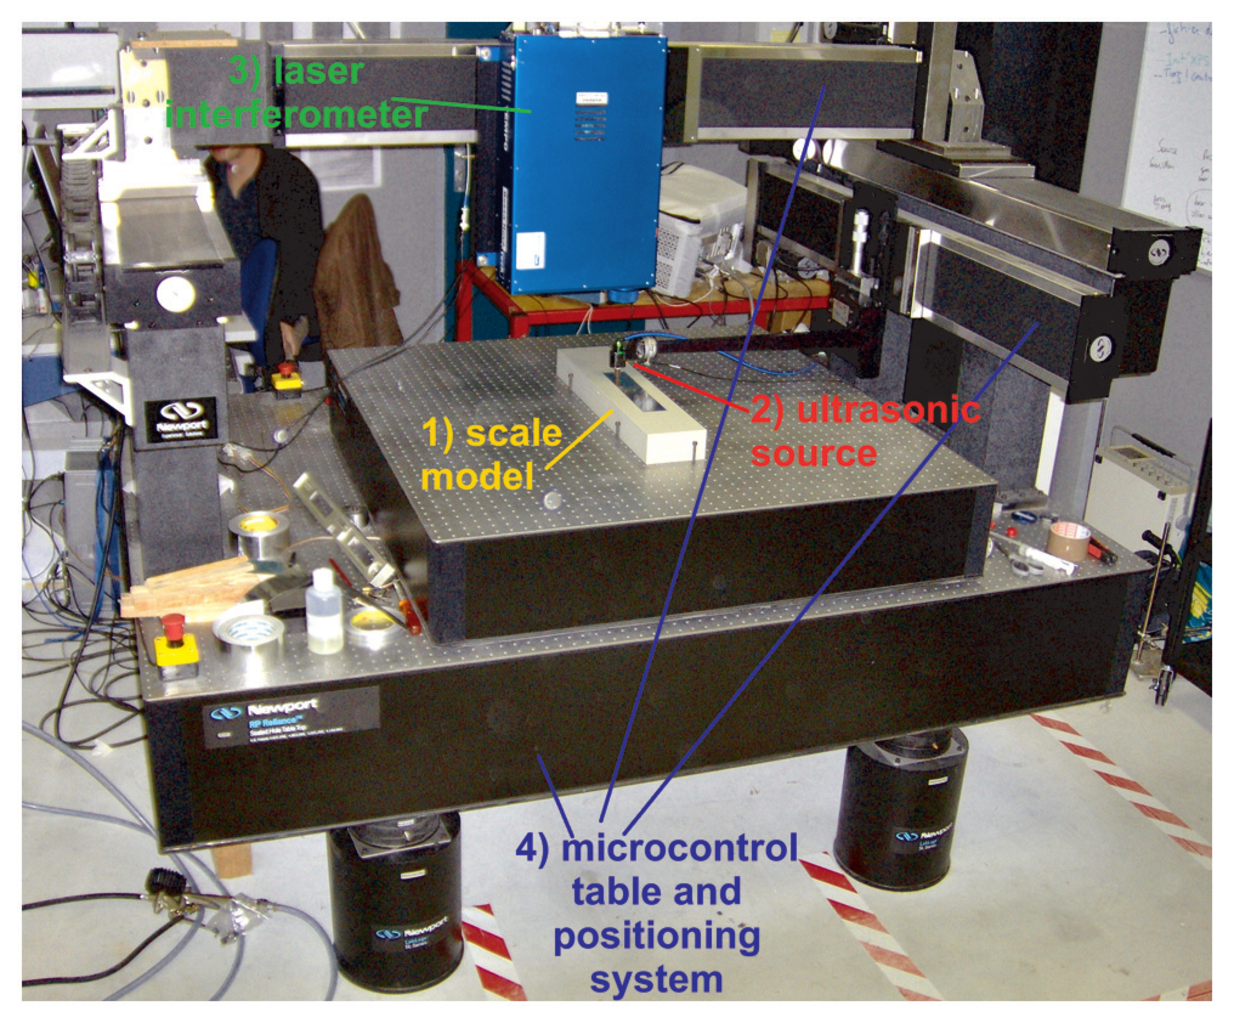
\includegraphics[scale=0.5]{fig/panel_musc_bench.eps}
	\caption{Photograph of the MUSC ultrasonic laboratory (from \citet{Bretaudeau_FWI_2013} )with its four components: (1) a small-scale model of the underground, (2) an optical table with two automated arms moving above the model, (3) a laser interferometer recording ultrasonic wave propagation	at the model surface,(4) a piezoelectric ultrasonic source generating ultrasonic waves in the model.}
	\label{panel_musc_bench}
\end{figure}

% #### Fig:: panl_multisrcrec
\begin{figure}[!h]
	\centering
	\includegraphics[scale=0.5]{fig/panel_multisrcrec.eps}
	\caption{Example of multi-source multi-receiver record on the MUSC system for a two-layer model (bialt).}
	\label{panel_multisrcrec}
\end{figure}

\begin{figure}[!h]
	\centering
	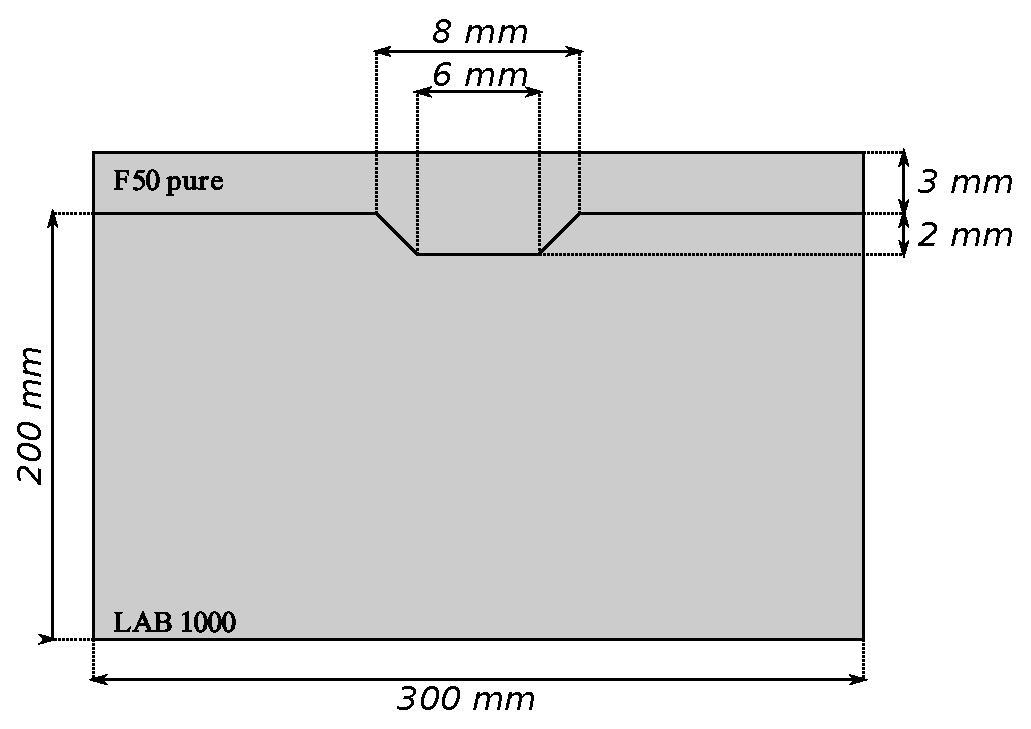
\includegraphics[scale=0.5]{fig/bialt_model.eps}
	\caption{Schematic representation of the so-called \textit{BiAlt} model.}
	\label{panel_bialt_model}
\end{figure}

% #### Fig:: piezo-source-validation
%\begin{figure}[!ht]
%	\centering
%	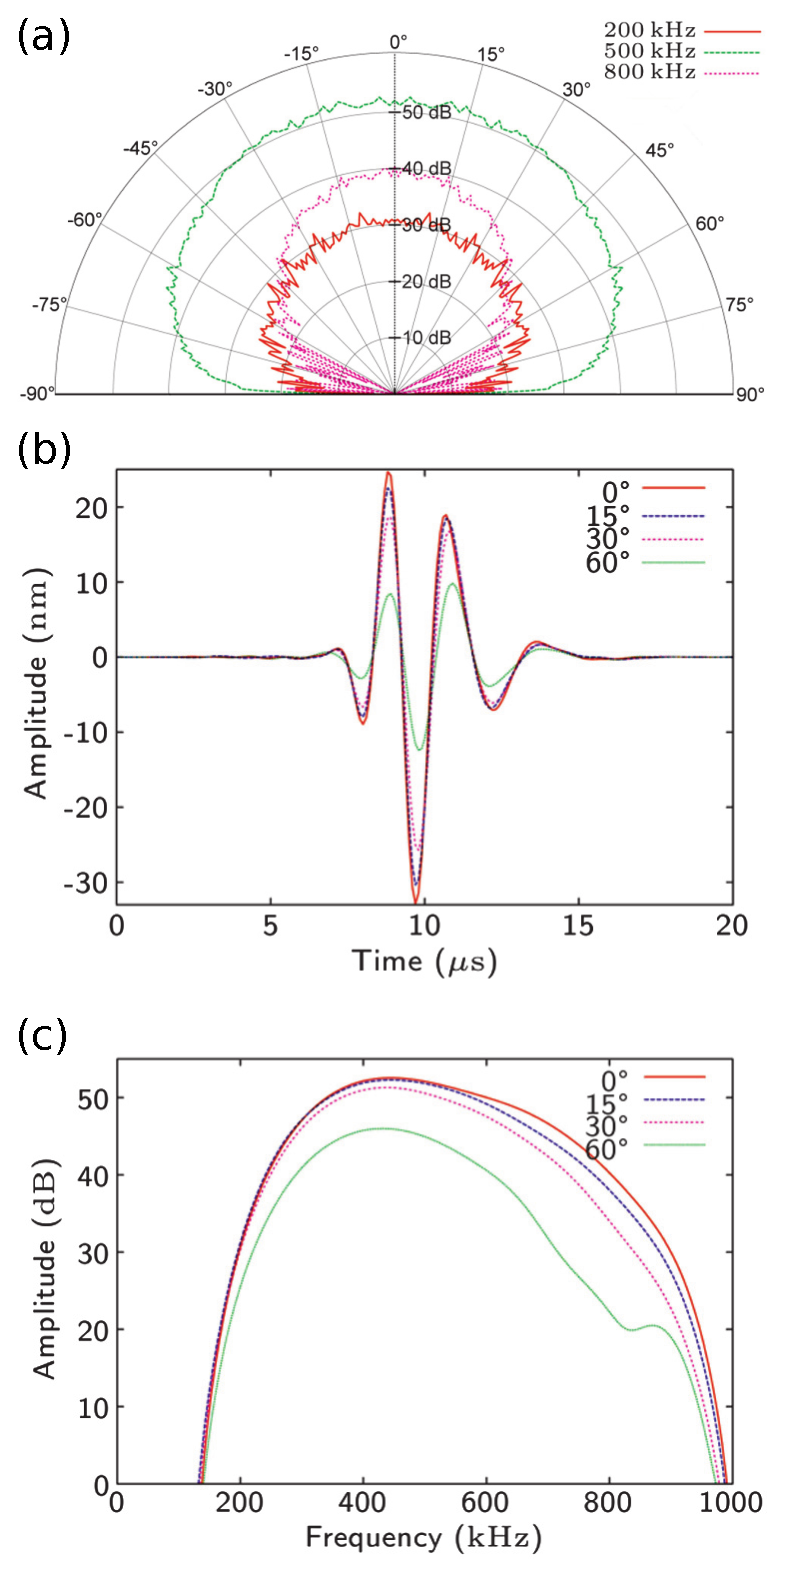
\includegraphics[scale=0.5]{fig/piezo-source-validation.eps}
%	\caption{Validation of the piezoelectric source coupled with an adapter \citep{Bretaudeau_SSM_2011}. (a) Directivity diagrams (dB) for the high-frequency source Panametrics\textregistered with conical polyurethane adapter: three frequencies — normal particle displacement. (b) Temporal signals and (c) amplitude spectrums for the high-frequency source Panametrics\textregistered with a conical polyurethane adapter in transmission through a PVC cylinder for	various angles of incidence: O, 15, 30, and 60 degrees — normal particle displacement.}
%	\label{piezo-source-validation}
%\end{figure}

% #### Fig:: panel_bialt_2d3d
\begin{figure}[!h]
	\centering
	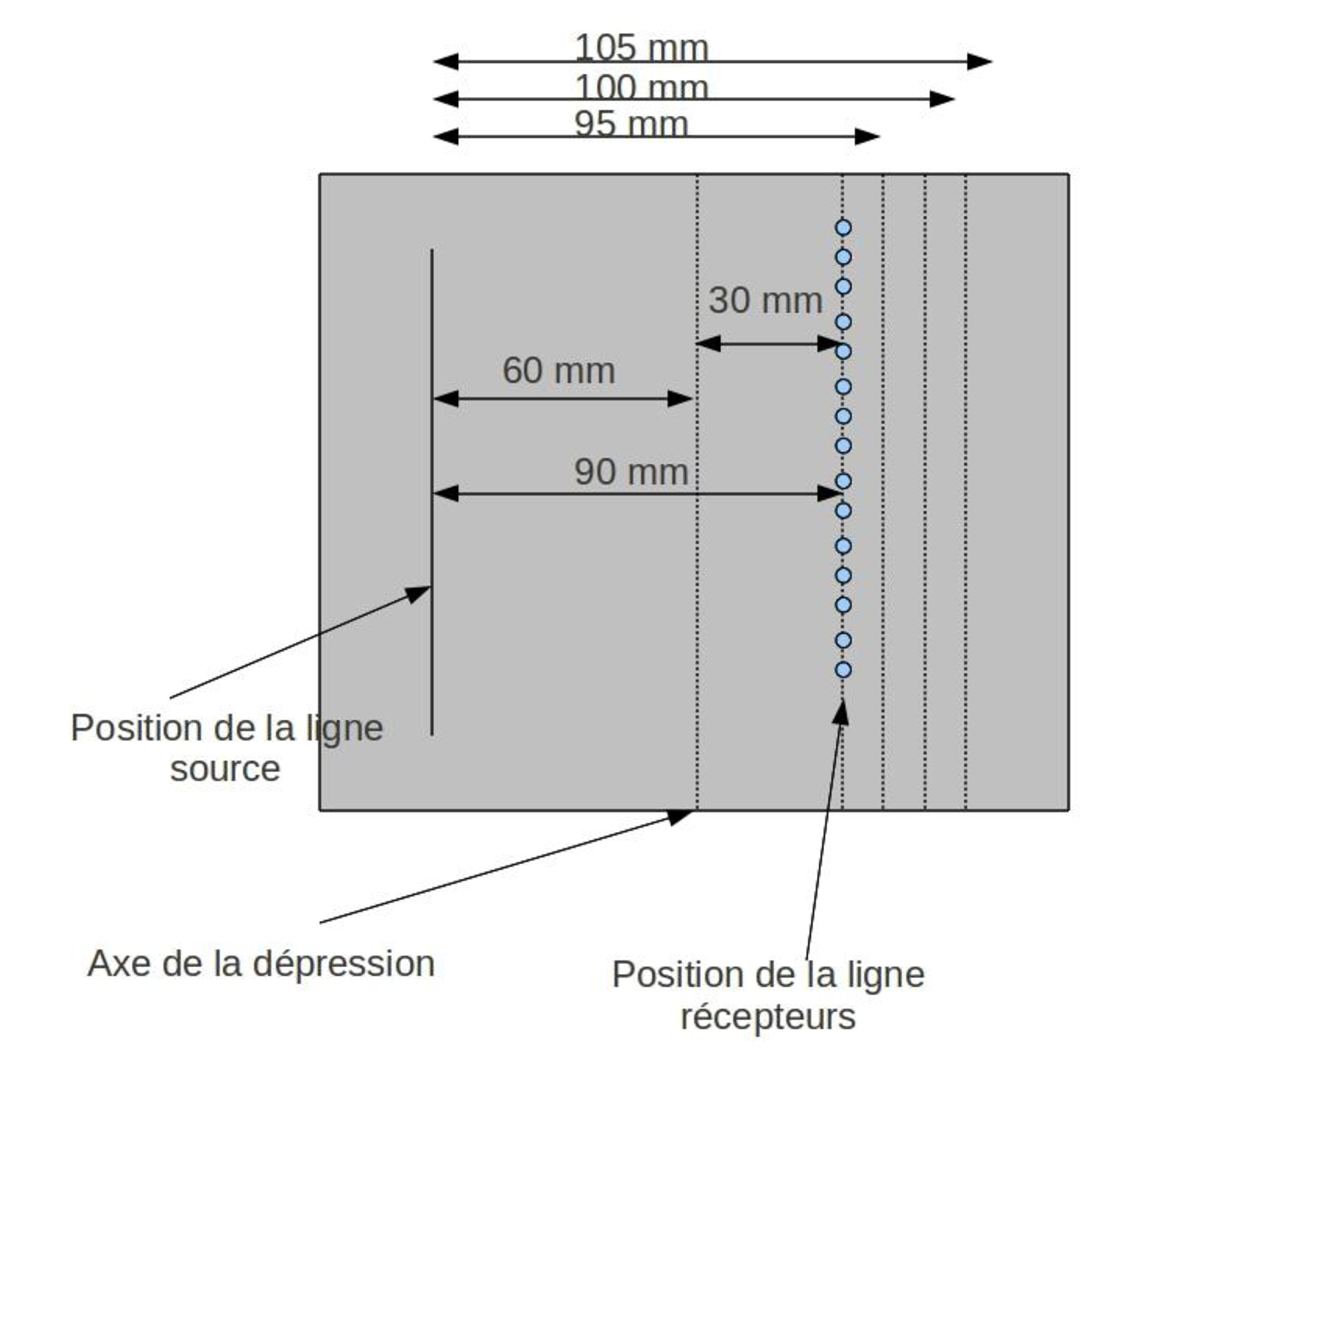
\includegraphics[scale=0.5]{fig/amplitude_acqui_principle.eps}
	\caption{Schematic representation of the acquisition geometry used to generate experimental line-source, \textit{i.e.} an equivalent of cylindrical source use in two-dimensional modeling. Black traingle and red circle represent receivers and sources, respectively.}
	\label{amplitude_acqui_principle}
\end{figure}

\begin{figure}[!h]
	\centering
	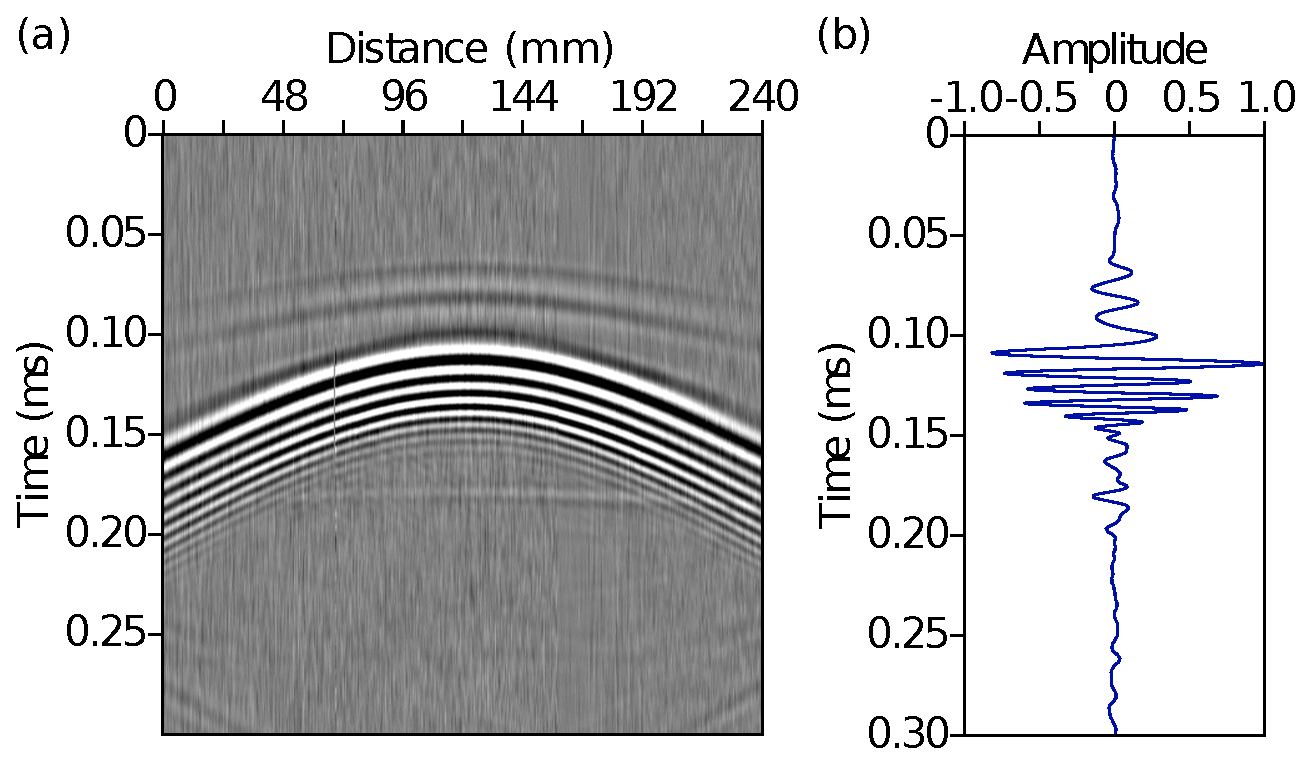
\includegraphics[scale=0.5]{fig/amplitude_stack_principle.eps}
	\caption{(a,b) Numerical modeling. (a) Resulting seismogram at one receiver position for the experimental line-source. (b) Comparison between point-source response in red (central trace of (a)) and line-source response in green (stack of (a)). (c,d) Same as (a) and (b) but for experimental modeling.}
	\label{amplitude_stack_principle}
\end{figure}

\begin{figure}[!h]
	\centering
	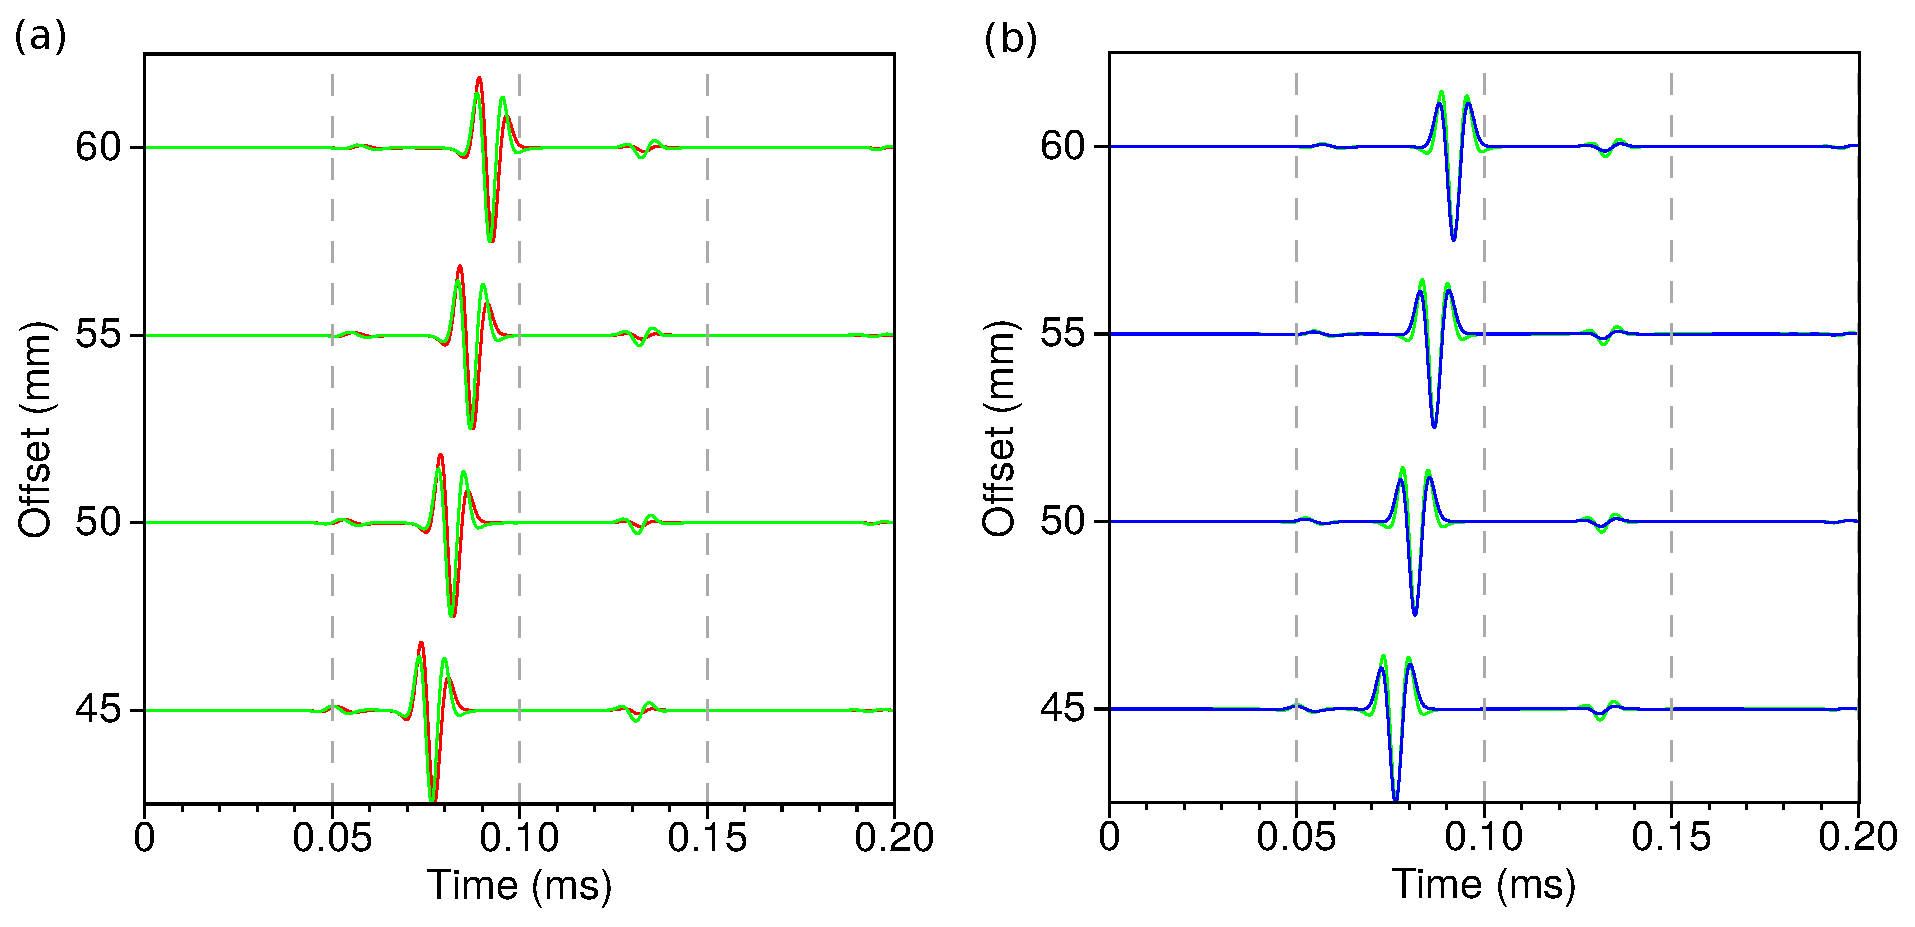
\includegraphics[scale=0.5]{fig/trans2d3d.eps}
	\caption{(a,b) Numerical modeling. (a) Comparison between synthetic seismograms for a point-source (red) and for a line source (green), for 45, 50, 55 and 60 mm source-receiver offsets respectively. (b) Comparison between synthetic seismograms for a line-source (green), and a point-source response corrected from geometrical spreading (blue) for same source-receiver offsets as (a). (c,d) Same as (a) and (b) for experimental modeling. The light-purple dotted lines pick $PSv$-wavefront.}%\textbf{cc} gives the correlation factor between line-source and point-source responses.}
	\label{panel_amplitude_sem}
\end{figure}

%\begin{figure}[!h]
%	\centering
%	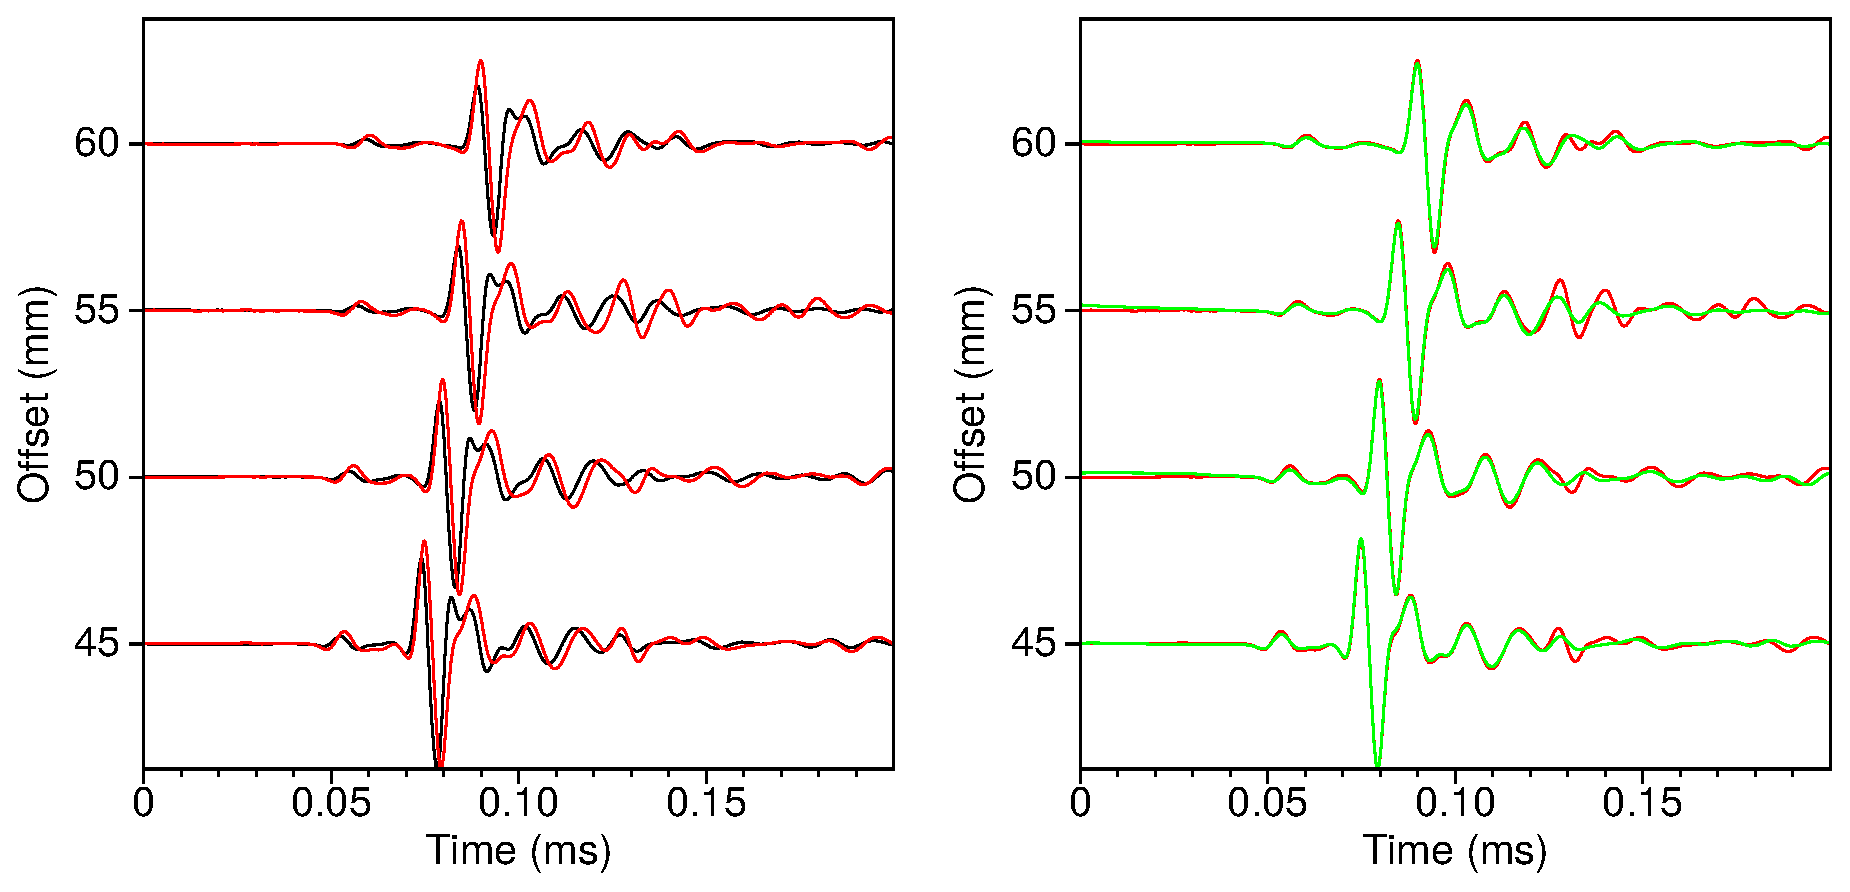
\includegraphics[scale=0.5]{fig/trans2d3d-musc.eps}
%	\caption{(a) Comparison between experimental seismograms for a point-source (red) and for a line source (black), for 45, 50, 55 and 60 mm source-receiver offsets respectively. (b) Comparison between experimental seismograms for a line-source (black), and a point-source response corrected from geometrical spreading (green) for same source-receiver offsets as (a).} %\textbf{cc} gives the correlation factor between line-source and point-source responses.}
%	\label{panel_amplitude}
%\end{figure}

% #### Fig:: panel_srcest_2d_mean
\begin{figure}[!h]
	\centering
	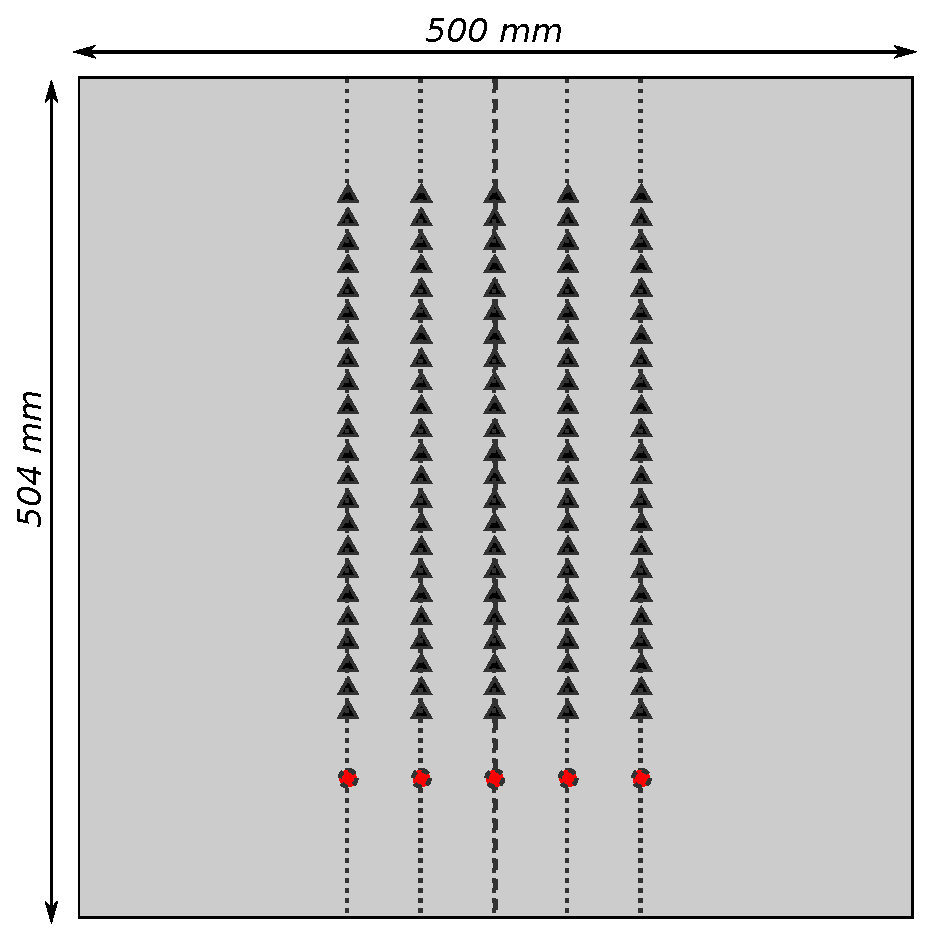
\includegraphics[scale=0.5]{fig/reproducibility_acqui_principle.eps}
	\caption{Schematic representation of the acquisition geometry used to assess the data reproducibility using the MUSC system. Black traingle and red circle represent receivers and sources, respectively.}
	\label{reproducibility_acqui_principle}
\end{figure}

\begin{figure}[!h]
	\centering
	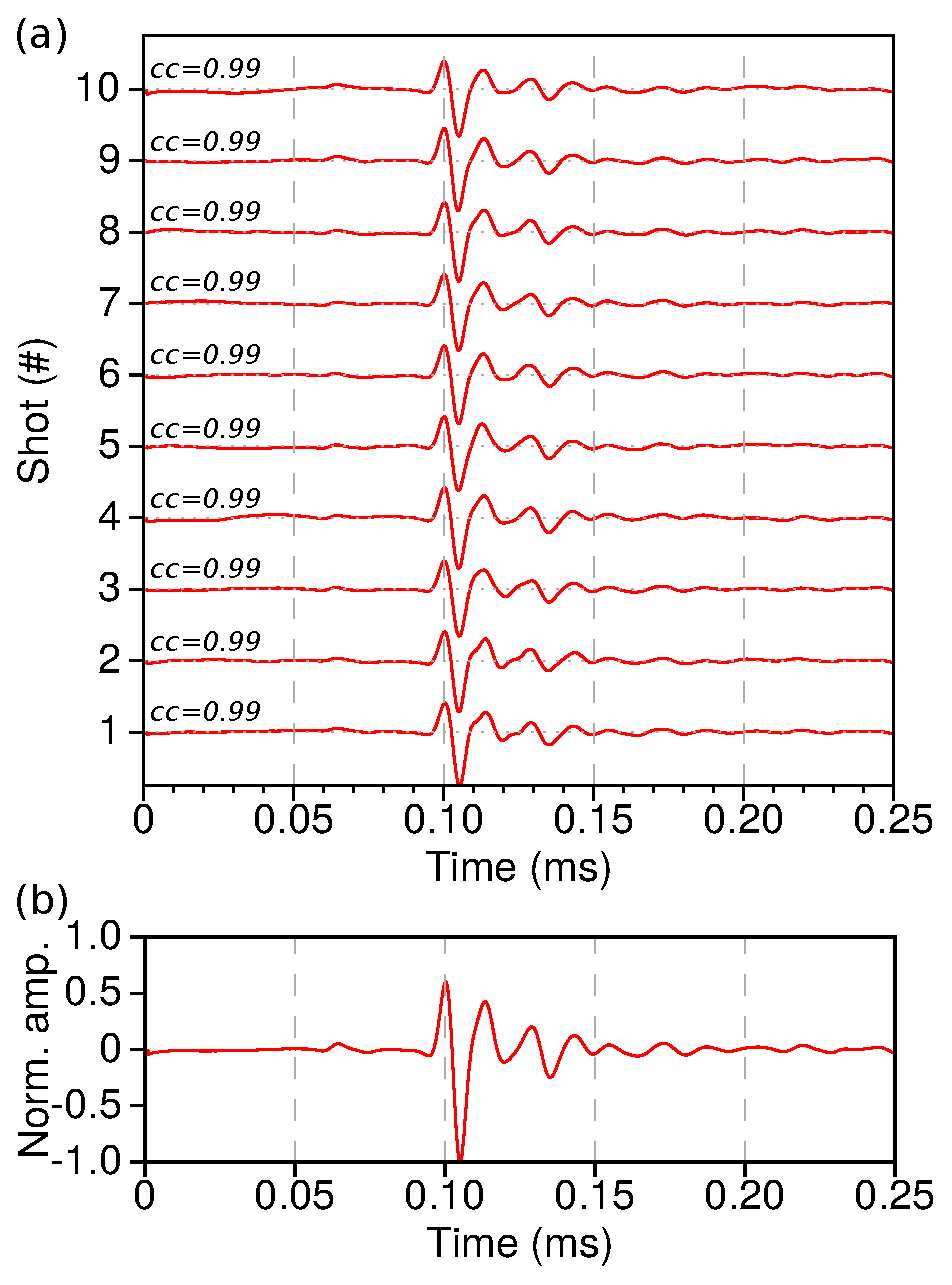
\includegraphics[scale=0.5]{fig/musc_F50_CT.eps}
	\caption{Central trace for each of the ten analogic experiment. \textbf{cc} gives the correlation factor of each central trace with respect to a mean trace.}
	\label{panel_central_traces_cc}
\end{figure}

\begin{figure}[!h]
	\centering
	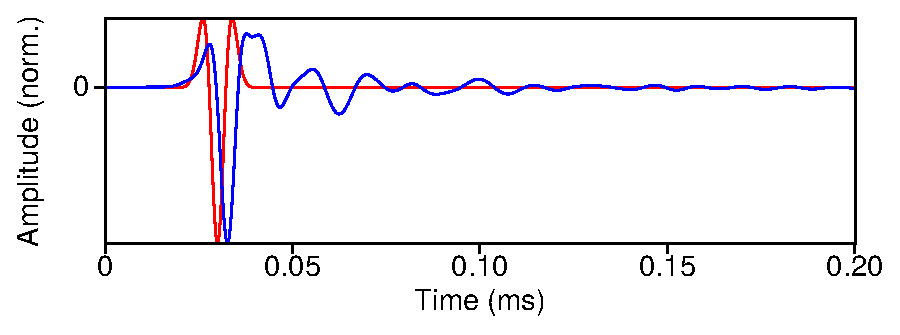
\includegraphics[scale=0.5]{fig/srccomp.eps}
	\caption{Comparison between the theoritical Ricker source send to the transducer and the effective source wavelet injected in the model.}
	\label{srccomp}
\end{figure}

\begin{figure}[!h]
	\centering
	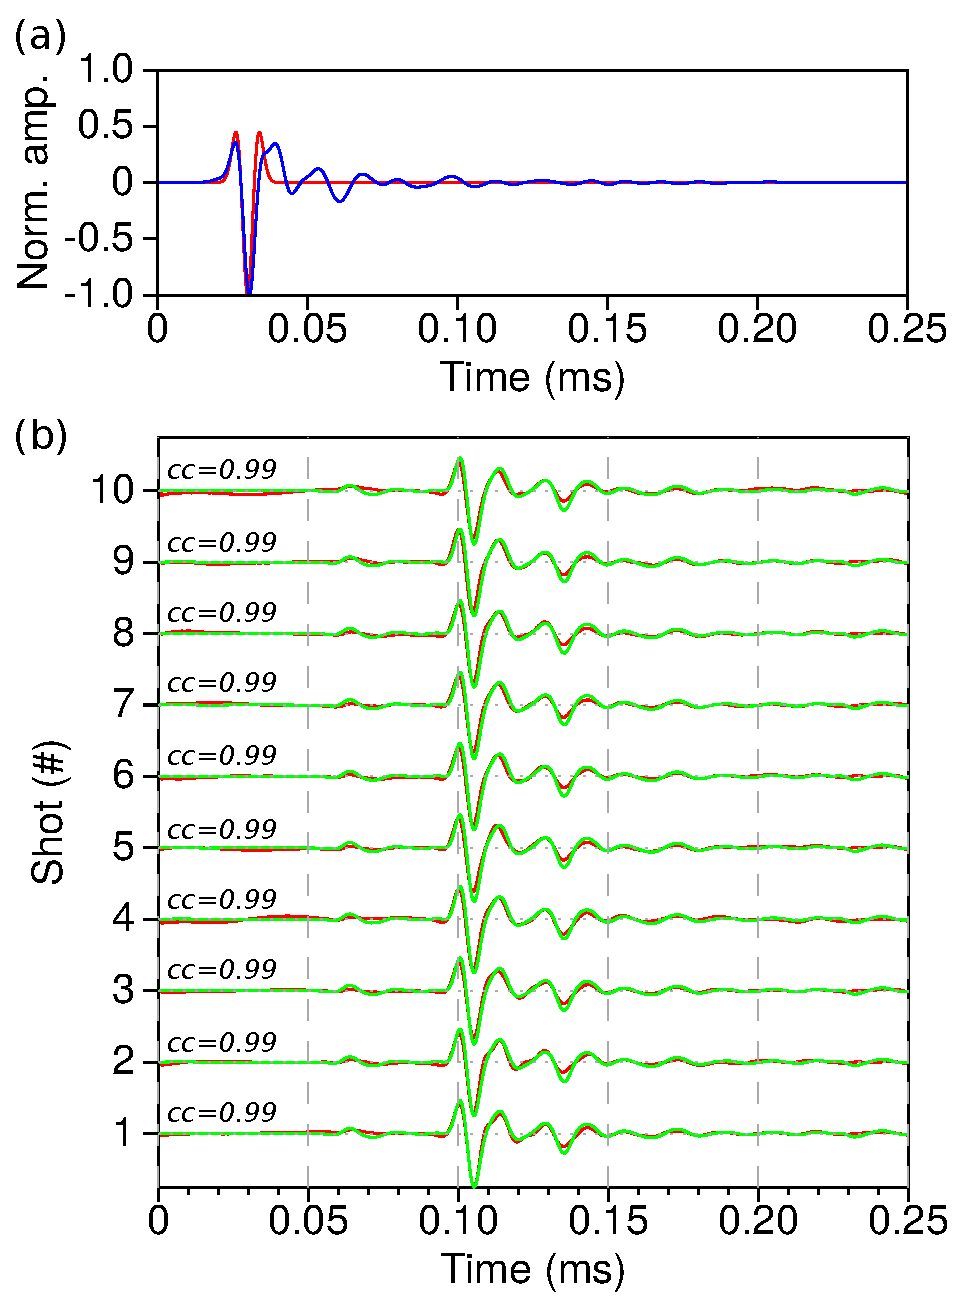
\includegraphics[scale=0.5]{fig/spec_F50_CT_COMP.eps}
	\caption{Comparison between analogic central traces (grey) and numerical traces corrected from the estimated effective source (black) for each experiment. \textbf{cc} gives the correlation coefficient.}
	\label{panel_srcest_2d_mean_comp}
\end{figure}

% #### Fig:: panel_bialt_model


\begin{figure}[!h]
	\centering
	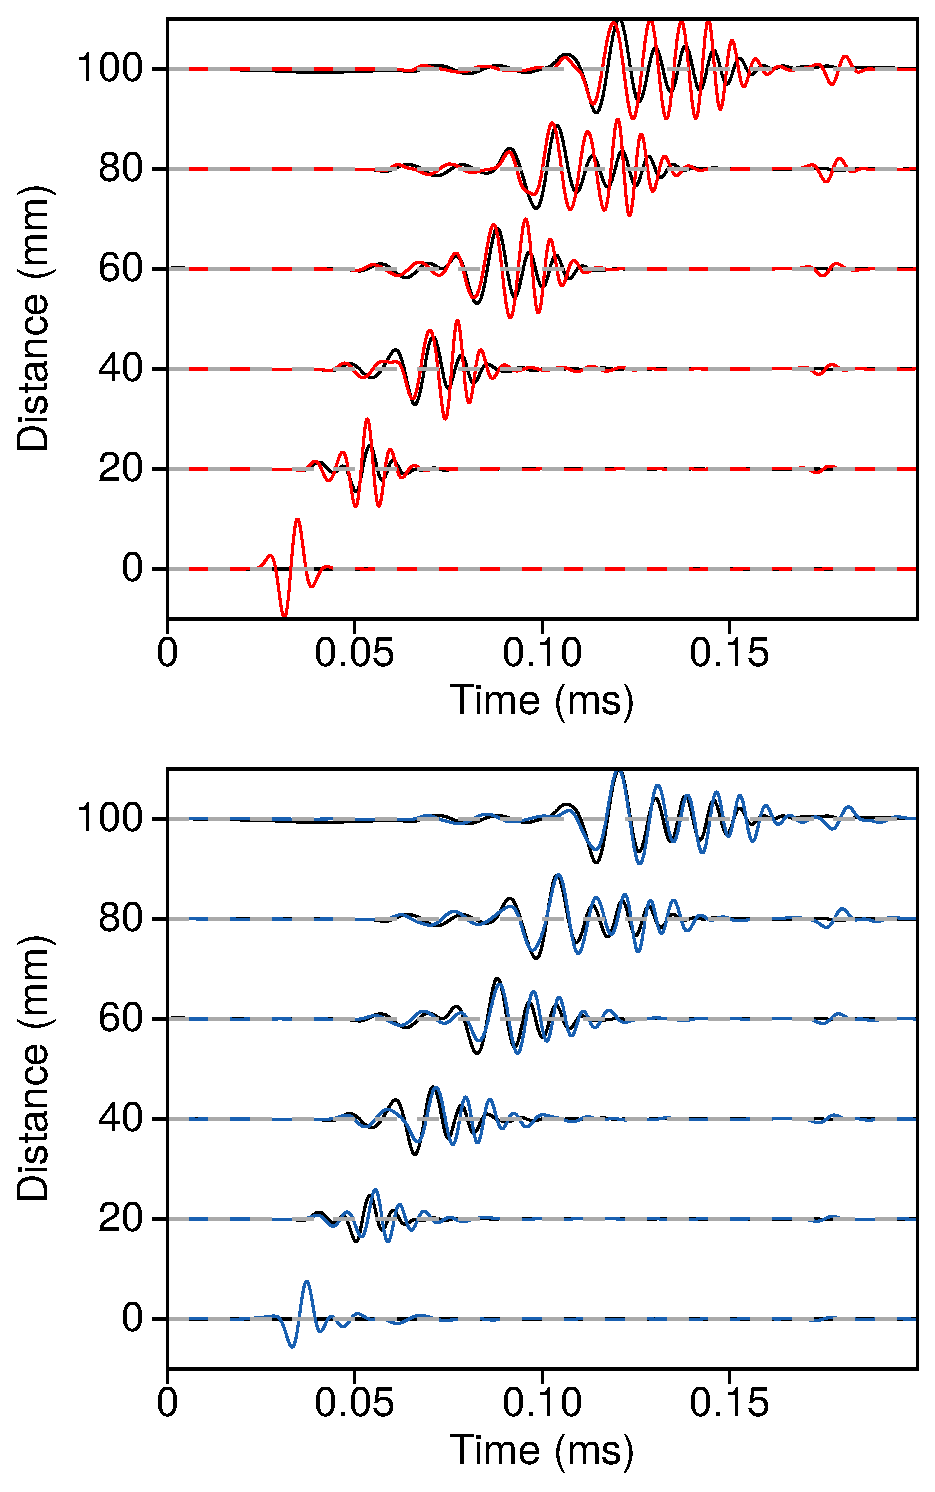
\includegraphics[scale=0.5]{fig/blind-comp-cor.eps}
	\caption{.}
	\label{blind-test}
\end{figure}

\clearpage
\newpage

\subsection*{Tables}

\begin{table}[!ht]
	\centering
	\begin{tabular}{cccccc}
		\hline
		material & $\mathrm{V_{P}\ (m/s)}$ & $\mathrm{V_{S}\ (m/s)}$ & $\mathrm{V_{R}\ (m/s)}$ & $\mathrm{\rho\ (kg/m^{3})}$ & $\mathrm{Q}$ \\
		\hline
		Aluminium & 5630 & 3225 & --   & 2700 & --  \\
		F50 pure  & 2300 & 1030 & 965  & 1300 & 30  \\
		F50 200\% & 2820 & 1425 & 1328 & 1766 & --  \\
		F50 240\% & 2968 & 1496 & 1388 & 1822 & --  \\
		LAB1000   & 2850 & 1400 & 1310 & 1500 & 75  \\
		\hline
	\end{tabular}
	\caption{Physical properties of some materials used to build small scale models. $\mathrm{V_{P}}$, $\mathrm{V_{S}}$ and $\mathrm{V_{R}}$ are the P-wave velocity, S-wave and the Rayleigh wave velocity, respectively. $\rho$ is the density and $\mathrm{Q}$ is the quality factor.}
	\label{epoxy-resin}
\end{table}

\begin{table}[!ht]
	\centering
	\begin{tabular}{|l|lcr|}
		
		\hline
		Distance               & $d_{real}\ (m)$            & $\rightarrow$ & $k^{-1}d_{reduc}\ (mm)$ \\
		Wavelength             & $\lambda_{real}\ (m)$      & $\rightarrow$ & $k^{-1}\lambda_{reduc}\ (mm)$ \\
		Time                   & $t_{real}\ (s)$            & $\rightarrow$ & $k^{-1}t_{reduc}\ (ms)$ \\
		Velocity               & $V_{real}\ (m.s^{-1})$     & $\rightarrow$ & $V_{reduc}\ (m.s^{-1})$ \\
		Density                & $\rho_{real}\ (kg.m^{-3})$ & $\rightarrow$ & $\rho_{reduc}\ (kg.m^{-3})$ \\
		Quality factor         & $Q_{real}$                 & $\rightarrow$ & $Q_{reduc}$ \\
		Particule displacement & $a_{real}\ (m)$            & $\rightarrow$ & $k^{-1}a_{reduc}\ (mm)$ \\
		Particule velocity     & $c_{real}\ (m.s^{-1})$     & $\rightarrow$ & $c_{reduc}\ (m.s^{-1})$ \\
		\hline
	\end{tabular}
	\caption{Scale ratio between viscoelastic parameters at the real scale and at a scale reduced by a coefficient $k$ (after \citet{Bretaudeau_SSM_2011}).}
	\label{scale-ratio}
\end{table}

\begin{table}[!ht]
	\centering
	\begin{tabular}{lcccc}
		\hline
		\qquad & 90 mm & 95 mm & 100 mm & 105 mm \\
		\hline
		$cc1_{init}$  & 0.702 & 0.725 & 0.728 & 0.728 \\
		$rms1_{init}$ & 0.794 & 0.760 & 0.762 & 0.774 \\
		\hline
		$cc1_{final}$  & 0.940 & 0.953 & 0.951 & 0.949 \\
		$rms1_{final}$ & 0.358 & 0.317 & 0.325 & 0.343 \\
		\hline
		\hline
		$cc2_{init}$  & 0.954 & 0.987 & 0.988 & 0.988 \\
		$rms2_{init}$ & 0.304 & 0.162 & 0.155 & 0.154 \\
		\hline
		$cc2_{final}$  & --   & --    & --    & --    \\
		$rms2_{final}$ & --   & --    & --    & --    \\
		\hline
	\end{tabular}
	\caption{.}
	\label{cc-rms}
\end{table}

\clearpage
\newpage 

\section{ACKNOWLEDGMENTS}

\clearpage
\newpage

\bibliographystyle{seg}  % style file is seg.bst
%\bibliography{/media/pageotd/1581-58C8/Work/git-repository//TR-VIBRIS/tail/bibvibris}
\bibliography{bibvibris,bibvibris_Dona,bibvibris-Dona,references}

\end{document}
